% Created 2023-02-15 Wed 15:15
% Intended LaTeX compiler: pdflatex
\documentclass[11pt]{article}
\usepackage[utf8]{inputenc}
\usepackage[T1]{fontenc}
\usepackage{graphicx}
\usepackage{grffile}
\usepackage{longtable}
\usepackage{wrapfig}
\usepackage{rotating}
\usepackage[normalem]{ulem}
\usepackage{amsmath}
\usepackage{textcomp}
\usepackage{amssymb}
\usepackage{capt-of}
\usepackage{hyperref}
\author{ambi}
\date{\today}
\title{Bracket Stamina: A Generalization of the Kelly Coin-Flipping Game to a Multiplayer environment}
\hypersetup{
 pdfauthor={ambi},
 pdftitle={Bracket Stamina: A Generalization of the Kelly Coin-Flipping Game to a Multiplayer environment},
 pdfkeywords={},
 pdfsubject={},
 pdfcreator={Emacs 26.3 (Org mode 9.1.9)}, 
 pdflang={English}}
\begin{document}

\maketitle
\tableofcontents


\section*{Abstract}
\label{sec:orgac327b4}

The Kelly Coin-Flip Game is a 300-round single player game where a player begins with \$25, and can bet any amount of their bankroll on a coin flip weighted 60\% favorably to earn a maximum of \$250. Most players fail to strategize well for this game, making it an interesting case study for irrational decision making. While generalizations of the Kelly Coin-Flip Game exist where the edge, the number of rounds, the ceiling and the starting value are all shifted according to various distributions both known and unknown to the player, all of these games focus on an iterative single-player setting where the object is to extract as much value as possible. Instead, we propose a variant which generalizes to a multiplayer, bracket-based environment. We study the properties of this game both in single- and double-elimination, as well as train a deep reinforcement learning agent whose performance in this multiplayer game (may or may not reveal similar inductive biases to humans? May reveal something interesting about theory of mind?)

\section*{The Multiplayer Variant}
\label{sec:orge8e7761}

\begin{center}
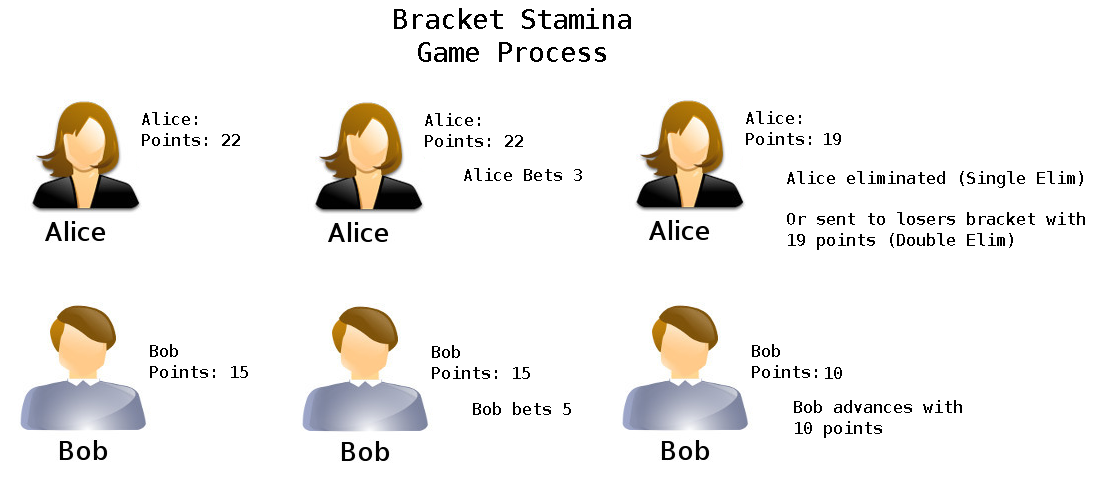
\includegraphics[width=.9\linewidth]{./bracketstam.png}
\end{center}

In Bracket Stamina, each player in a 16-man bracket begins with 25 points (or dollars). Two players in each round face off and provide a value of points they wish to “bet”. Once the bet has been placed, both players lose that number of points. If a player's bet is higher than the opponent’s, that player will advance to the next round. If it is lower, the player is eliminated from the single-elimination setting, or sent to losers bracket in the double elimination setting, with those “bet” points still lost. If the value is the same, a winner is randomly determined. We study two rewards structures: one which rewards players for high placement (e.g. 5th gets paid out more then 9th), and one which rewards players for winning (e.g. winner takes all)

This game has all of the critical elements of the Kelly Coin-Flip game: a pre defined maximum number of rounds which can be reached early through losing, an “edge” represented by the selected point differential, the earnings ceiling (winning the tournament), and a known a priori starting points value (or perhaps distribution). What we have added is the strategic element of another agent: where each agent is incentivized to win as narrowly over its opponents as possible, to save as many points as possible for the final round, where it should spend everything. How do people perform on this? How should agents?

\section*{What Could We Find?}
\label{sec:orga668e32}

Unlike the original Kelly Coin-Flip Game, this game does not immediately appear to have a "winning" strategy, since the other agent could construct a strategy to defeat yours. That is, it may be a game for which diverse strategies all emerge as "viable" depending on the distribution of strategies and goals held by other agents. A winning strategy developed where all opponent agents select a random value may not hold against a winning strategy held where all opponent agents use that same strategy.

Humans are known to have interesting behavioral processes in elimination tournaments (e.g. the stronger the next round opponent is, the less likely it is that the stronger player wins the current round's match), and it's possible that we could learn some interesting human-held heuristics about resource conservation and modeling the intent of other agents' resource conservation. 

It's also unclear whether or not self-play is an appropriate paradigm for learning this game, as is usually done in most other deep RL paradigms. As mentioned, it seems feasible that "off-meta" or "adversarial" strategies could be constructed around defeating the current "meta" strategy with high likelihood, in a similar manner to adversarial policies that can handily defeat superhuman go AIs and yet lose horribly to human players. Difficulty optimizing RL agents could point to some strong human-held heuristics for these sorts of problems.

\section*{Some Useful References}
\label{sec:org0d91614}

Gwern Deep RL on the kelly coin-flip game: \url{https://www.gwern.net/Coin-flip}

Selecting the Best: Spillover/Shadow effect in elimination tournaments: \url{https://www.nber.org/papers/w17639}

Jon Bois - The NCAA is a loser machine (Unusual properties of elimination brackets): \url{https://youtu.be/4a1TUszkMfI}

adversarial policies beat superhuman go AIs \url{https://arxiv.org/abs/2211.00241}
\end{document}
